\documentclass[hyp]{socreport}
\usepackage{fullpage}

\usepackage{url}
\usepackage{amsmath,amsthm,amsfonts}
\usepackage{algorithm,algorithmic}
\usepackage[dvips]{color}
\usepackage{algorithm,algorithmic}
\usepackage{graphicx}
\usepackage{CJKutf8}

\usepackage{tikz}
\usetikzlibrary{trees}
\usetikzlibrary[positioning]
\usetikzlibrary{calc}
\usetikzlibrary{decorations.pathmorphing}
\usetikzlibrary{fit}
\usetikzlibrary{backgrounds}
\tikzstyle{level 1}=[level distance=4cm, sibling distance=3.5cm]
\tikzstyle{level 2}=[level distance=4cm, sibling distance=2cm]
\tikzstyle{bag} = [text width=4em, text centered]
\tikzstyle{end} = [circle, minimum width=3pt,fill, inner sep=0pt]
\tikzstyle{fork} = [circle, minimum width=3pt,fill, inner sep=0pt]

\begin{document}
\pagenumbering{roman}
\title{Word Sense Prediction Using Decision Trees}
\author{Heng Low Wee \\ (U096901R)}
\projyear{2010/11}
\projnumber{U079330}
\advisor{A/P Min-Yen Kan}
\deliverables{
	\item Report: 1 Volume
	\item Source Code: 1 DVD}
\maketitle
\begin{abstract}
\paragraph{}
%%%From Aobo: Better to show the motivation of reducing the size and time, which is to make it more applicable in a real time software like DICE translator.
%%% updated
Word sense disambiguation (WSD) is a key task in Natural Language Processing. There are many existing systems that are able to achieve good performance in \textsc{SensEval} and \textsc{SemEval} tasks. However, few systems discuss about reducing the size of the training model and the time taken for the WSD process. For WSD systems to be applied onto real-time softwares, such as building a WSD software for mobile devices, they need to be scaled down in terms of its training model size, and be responsive to enhance user experience. With that, we propose the idea of building a WSD system that is light-weight and speedy.

\paragraph{}
%%%From Aobo: maybe indicate what is the data size and processing time before reducing, or show how many percentage it has reduced.
%%% updated
In this report, we study how we can adopt using Decision Trees to predict the word senses of ambiguous words. Our system aims to reduce the size of the training model and the time taken to predict word senses. In our implementation, we reduced both the size of our training model and the time taken by over 98\%, with our system performing speedily when disambiguating sentences, while retaining a reasonable performance for accuracy.

\begin{descriptors}
	\item I.2.7 Natural Language Processing
\end{descriptors}
\begin{keywords}
	decision tree,  word sense disambiguation, word sense, ambiguous
\end{keywords}
\begin{implement}
\begin{flushleft}
\hspace{5 mm}Software: Java, Perl, Weka 3.\\
\hspace{5 mm}Hardware: MacBook Pro, Intel Core 2 Duo 2.4GHz, 4GB Memory.
\end{flushleft}
\end{implement}
\end{abstract}

\begin{acknowledgement}
\paragraph{}
First of all, I would like to thank my supervisor, A/P Min-Yen Kan, for his support throughout the entire duration of this project. He was very patient, and always willing to answer my questions whenever I had any doubts. He also gave me advices on the project, and suggestions on how to make things better.

\paragraph{}
I am grateful to be offered this opportunity to participate in such a research project and be able  to meet and work with members of Kan's research group, WING. I would like to thank the WING group for their advices during my practice talk sessions with them. On top of that, I would like to thank Wang Ao Bo and Chen Tao, for their advices and for their time spent on helping me make this report better.
\end{acknowledgement}

\listoffigures
\listoftables
\tableofcontents

\chapter{Introduction}
\label{introduction}
\paragraph{}
In the English language, there are many words and even phrases that have multiple interpretations depending on the context. These words have multiple \textit{senses} or meanings, and are ambiguous. For instance:
\begin{enumerate}
\item She is interested in the \textit{interest} rates of the bank.
\item He developed an \textit{interest} in art.
\end{enumerate}

\paragraph{}
It is not difficult for a human to see that the word \textit{interest} has different meanings in the two sentences. We humans are able to determine the context of each sentence immediately, and hence able to identify the correct sense for the ambiguous word. A machine, however, needs to run through a series of analytical processes before it can determine the best answer. This process is termed Word Sense Disambiguation (WSD). More formally, WSD is the process of deciphering the intended meaning of an ambiguous word in a given context.

\paragraph{}
%%%From Aobo: "such as machine learning" ml is not an example of application.  machine translation?
%%% updated
WSD is a key task in Natural Language Processing. It has many applications in computational linguistics, such as machine translation, text mining and information retrieval. It can also be applied within search engines such that the search results will be more relevant, when the results have the same intended meaning as the search query.

\paragraph{}
There are four conventional types of WSD, they are:
\begin{enumerate}
\item Dictionary-based \& knowledge-based \\
This method uses formal dictionaries and lexical knowledge bases as their primary source to disambiguate senses. Dictionaries provide the definitions of the possible senses of an ambiguous word. The definitions can then be used in WSD algorithms. One example is the Lesk Algorithm \cite{lesk}, that words in a given environment (sentence, paragraph etc) will tend to share a common topic. Banerjee \& Pedersen, instead of using standard dictionaries,  used WordNet \cite{wordnet} as a sense inventory in their implementation of the Lesk Algorithm. WordNet is arranged semantically, creating an electronic lexical database that provides a rich hierarchy of semantic relations that can be exploited. The authors exploited this advantage of WordNet and integrated into the Lesk Algorithm. They found that the adapted implementation outperformed the traditional Lesk approach with double the accuracy.
%%From Chen Tao:The whole paragraph emphasizes the use of dictionaries (formal or informal), but not mention much about knowledge bases. Can I just understand that dictionaries also provide lexical knowledge? It will be better if introducing the relationship between dictionary-based and knowledge-based method.
\item Supervised \\%%From aobo : maybe need reference for this paragraph. and the first sentence is not definitely correct.
% updated
Supervised WSD uses manually sense-tagged corpora as their primary resource to perform WSD. It can be formulated as a classification problem where word senses represent classes and a classifier assigns a class to a new instance of a word. Some classifiers are the Naive Bayes, Decision Lists \cite{supervisedmethods} and Support Vector Machines \cite{svm}.
%Support Vector Machines have been known to be one of the most successful approaches for WSD because they can cope with high-dimensionality of the feature space.
\item Semi-supervised \\
This method makes use of both labeled and unlabeled data. Similarly, it refers to using multiple untagged corpora to provide concurrent information to supplement a tagged corpus.
\item Unsupervised \\
Most challenging approach among all, this method may also be related to \textit{Word Sense Induction}, where senses could be induced by analyzing words in a given text. Unsupervised methods perform WSD with minimal, or no, dependence on sense-tagged corpus. \cite{noisy} described a probabilistic approach based on the Noisy Channel Model that uses an unlabeled word corpus derived from publicly-available web pages. Their system outperformed all the unsupervised systems compared with, some of which the authors claimed that they should be classified as semi-supervised instead.
\end{enumerate}

\section{Motivation}
%%From Aobo: your contribution is the balance between efficiency and accuracy, so the motivation should mention the balance beside simply benefiting MT.
%updated
\paragraph{}
There are many WSD systems that can provide great accuracies in disambiguating words. However, most of these systems are also not publicly available, either for its applications or for further research. Also, these systems are not suitable to be deployed as real-time softwares, such as for use on mobile devices, as the size of their training models are relatively large to be suitable.

\paragraph{}
The motivation in this project, other than to encourage the usage of WSD applications, is to build WSD systems that are small, and responsive such that they are more suited to be deployed on mobile devices or web browsers.

%\paragraph{}
%The motivation in this project is its benefits when applied into bilingual translation. For instance, English to Chinese. Consider this example:
%\begin{center}
%He developed an \textit{interest} in art.
%\end{center}
%\paragraph{}
%In this context, we can see that the word \textit{interest} is more related to the word ``hobby''. So when we translate the word \textit{interest} from English to Chinese, the correct output would be \begin{CJK}{UTF8}{gbsn}兴趣\end{CJK} (a person's interest) instead of \begin{CJK}{UTF8}{gbsn}利息\end{CJK} (simple interest). Being able to translate while retaining the original context would definitely prove to be more relevant for the end-users. Furthermore, this would encourage language learning as it is simpler and more straightforward when a learner is aware of which is the correct sense to be used in a given context.

%\paragraph{}
%In this paper, however, we do not venture into the field of translating the words into a second language. Instead, we focus on studying how we can predict the word senses of ambiguous words in the English language.

%%%From Aobo: before performance indicators, a chapter explaining what your approach(DT) is and why you use this approach(DT) is needed.
% updated
\section{Goals}
\paragraph{}
In this project, we explore how we can build a system that is small, suited for real-time applications. For that, we have considered three goals to measure the performance of our system in this project. They are:
\begin{enumerate}
\item Accuracy - percentage accuracy in predicting word senses
\item Speed - time taken to predict word senses and return the results
\item Size of Model - size of the training model used by the system to predict word senses
\end{enumerate}
\paragraph{}
We intend to build a system that is meant to perform WSD on small amount of text, like a sentence. One application for such a system is a language-assistance based tool to be integrated with web browsers, like a plugin in Firefox, so that users are able to find out more information, like pronunciation and definition, about some words on the web page by selecting the text using the mouse. WSD comes into the picture as we see the need for these information to be context-relevant from where the selected text is from. However we must keep the response time small, so that we can maintain user's experience. One can imagine an user who has the habit of selecting text on web pages very often. Any language tool with slow response will be not ideal.

\paragraph{}
For that, as much as possible, we intend to keep the model size as small as possible, while retaining a reasonable level of accuracy. We want it to be speedy and responsive. Also, we hope to reduce the amount of pre-processing prior to the prediction of word senses. We believe that by including too many pre-processing features, the system would require additional supporting files that could be significant in terms of file size. 
\chapter{Related Work}
\label{Related Works}
\section{Citation Analysis}
\paragraph{}
Several authors had researched on works related to citation analysis. In these works, they could be categorised into several directions for development. One of them that has a major impact would be citation classification or similarly, the classification of citation function. This task is aimed at making sense of the rationale why the authors of a paper would cite the work of another, and thus better aid readers on understanding the key ideas presented in a paper. The reasons why authors would cite, are what was meant by the citation function. In an updated version of their paper, Teufel et al. presented an annotation scheme for annotating a citation's function \cite{teufel2009annotation}. In their scheme, citations are generalised into 4 main categories: Weak, Contrast, Postive \& Neutral. Some of these categories are further broken down into more specific sub-categories, producing a total of 12 classes for annotating citations. \cite{teufel2006automatic} had already worked on the automatic classification of citation function, utilising features extracted from the \textit{citing context}. \cite{dongensemble} presented an approach to citation classification that uses a combination of various supervised learning algorithms. Similarly, authors worked on analysing the sentiment of citations to determine the polarity of these citations. \cite{athar2011sentiment} used sentence structure based features extracted from the citing context and produced promising results.

\paragraph{}
In \cite{citation-sensitive} and \cite{csibs}, Wan and his teams worked on building a research tool that acts a reading aid for readers when browsing through scientific papers. Wan et al. investigated the \textit{literature browsing task} by conducting surveys on researchers who read scientific papers frequently to update themselves. In this initial study conducted by Wan et al., several key ideas were revealed. First, when researchers read scientific papers and see citations made by the author, their main concern, as time-constrained professionals, is whether the cited paper would be worth their time and effort, and money, to follow up on and at the same time, whether to believe in the citation. Second, readers faced the difficulty of finding the exact text that justify the citation. Third, the surveys revealed that readers found it useful if a reading tool could identify important sentences and key words in the cited paper. This study conducted by Wan et al. is based on the fundamental idea of improving the reading experience of practitioners and researchers. The goal is to save a reader's time by helping the reader make relevance judgements about the cited documents. As it is often that readers have to read up on the cited documents to gain a better insight on the current context, this task would be of relevance. The authors then developed the CSIBS based on their studies. The CSIBS tool helps reader determine whether to read on the cited papers by providing a contextual summary of the cited papers.

%Tao: Could you show the reasons of reviewing sentence alignment, that is, the connection/similarity between citation provenance and sentence alignment? 
\section{Sentence Alignment}
\paragraph{}
Aligning sentences belonging to similar documents of the same language is an important research area for tasks related to summarisation and paraphrasing. \cite{nelken2006towards} presented a novel algorithm for sentence alignment in monolingual corpora. They showed their approach, which is based on TF*IDF similarity score, produced great precision at aligning sentence, with precision score of 83.1\%. A more recent work by \cite{li2010fast} introduced a new sentence alignment algorithm called Fast-Champollion. Briefly, it splits the input text into alignment fragments and identifies the components of these fragments before aligning them using a Champollion-based algorithm.





\chapter{Our Approach}
\label{approach}
\section{Terminology}
\paragraph{}
To aid the reader, and to avoid misunderstanding and confusion, it is important that we first list some of the key terms we are using in our paper.
\begin{table}[h]
	\center
	\begin{tabular}{ l p{13cm}}
		\textsc{Term} & \textsc{Description}\\
		\hline
		Citing Paper & The paper that makes the citation \\
		Cited Paper & The paper that is being cited by the citing paper \\
		Cite Link & E.g. \url{E06-1034==>J93-2004}. A citation relation between a citing paper (\url{E06-1034}) and a cited paper (\url{J93-2004}) \\
		Cite String & The citation mark. E.g. Nivre and Scholz (2004), [1], (23) \\
		Citing Sentence & A sentence in the citing paper that contains the in-line citation. E.g. \textit{That algorithm, in turn, is similar to the dependency parsing algorithm of \textbf{Nivre and Scholz (2004)}, but it builds a constituent tree and a dependency tree simultaneously.} \\
		Citing Context & The block of text surrounding the citing sentence, about 2 sentences before and after the citing sentence, for providing contextual information \\
		Cited Fragment & A fragment, from a few lines to paragraphs, in the cited paper
	\end{tabular}
	\caption{Terminology}
	\label{tab:terminology}
\end{table}

\section{Problem Analysis}
\subsection{Types of Citation}
\paragraph{}
In the scope of our project, all citations are classified into 2 types: \textbf{General} and \textbf{Specific}. We define citations as such to be inline with our goal. That is, to be able to tell, if Specific, where the cited information is in the cited document. Otherwise, the citation would be deemed General. To rid of ambiguity in our definition of a General/Specific citation, we have the following guidelines:\\
\textbf{General Citations}
\begin{enumerate}
\item Authors may refer to a paper as a whole. If the author cites for a key idea, e.g. Machine Learning, and Machine Learning makes up the entire or majority of the cited paper, it is a general citation.
\item Authors may refer to a paper as a form of mentioning. The authors merely mentions the cited paper out of acknowledgement of its contributions.
\end{enumerate}
\textbf{Specific Citations}
\begin{enumerate}
\item Authors may refer to a term definition in the cited paper.
\item Authors may refer to a key idea/implementation in the cited paper. This key idea/implementation does not make up the entire cited paper.
\item Authors may refer to an algorithm or a theorem in the cited paper. This algorithm/theorem does not make up the entire cited paper.
\item Authors may refer to digits or numerical figures in the cited paper. Usually for making reference to evaluation results in the cited paper. Authors may also complement the cited paper for its promising/excellent performance.
\item Authors may quote a line/segment in the cited paper.
\end{enumerate}
\paragraph{}
In general, for \textbf{Specific} citations, we would be able to specifically extract a fragment in the cited paper that represents the source of the information mentioned in the citation itself i.e. Citation Provenance.

%Tao: Could you remove/combine some of the subsection titles? Since some subsection only consist of 1 or 2 paragraphs.
\subsection{Locating The Cited Information}
\paragraph{}
Our problem is now reduced to determining whether a citation is General or Specific. If a citation is General, the reader can be directed, for example, to the Abstract section of the cited paper, but this is not the main focus of our task. If a citation is Specific, the reader can be directed to that specific paragraph or lines respectively. Therefore during computation, the cited document can be broken down into fragments. Hence if given that a citation is Specific, then there must exists a fragment that the citation refers to. For this we need to implement some ranking system that determines the location of this fragment.

\subsection{Scope Of The Problem}
\paragraph{}
In this project, we abstract away the problem of locating the in-line citations in a paper, and reduce our problem to only determining the type of a citation and its location. To solve the problem of locating the in-line citations, we utilize the open-source ParsCit system developed by \cite{parscit}. Conveniently, ParsCit identifies the citing sentence, together with the citing context.

\subsection{Modelling The Problem As Search}
\paragraph{}
In web search engines, an user enters a search query, and a search engine would use this query to search within its search domain -- millions of web pages -- and then display the best matching web pages as compared to the search query. That would be equivalent to having a search query for an entire corpus of research papers. Our problem can also be modelled as a searching problem, but a reduced version as compared to web search engines.

\paragraph{}
Consider reading a paper, \url{A}. We know the citations made by \url{A}, and these cited papers are listed in the References section of \url{A}. From this our search domain for any query from \url{A} would be the contents of the list of cited papers. We reduce this search domain further when we are investigating a particular citation in \url{A}, say now paper \url{A} cites the paper \url{B}. Now, for this citation, the scope of search would be the sub-domain -- contents of paper \url{B}. So instead of searching for the best matching document in the corpus, we are now searching within \url{B}. Our problem analysis tells that we have to break down \url{B} into fragments, and the search query would be for these fragments (Refer to Figure \ref{fig:model} for a simple illustration). With the help of ParsCit \cite{parscit}, the citing context can be extracted. The search query would be citing context which consists of the citing sentence.

\begin{figure}[h]
  \centering
  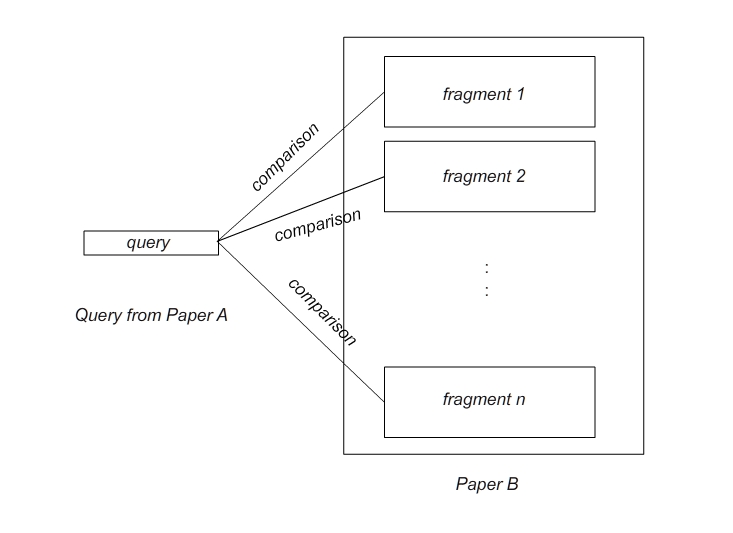
\includegraphics[scale=0.50]{./model}
  \caption{Modeling Our Problem}
  \label{fig:model}
\end{figure}

\paragraph{}
Our problem is now a \textit{binary classification problem}, where we attempt to determine whether a fragment is either General or Specific.

\section{Training Corpus}
\paragraph{}
At this initial stage, we picked the ACL Anthology Reference Corpus\footnote{http://acl-arc.comp.nus.edu.sg/} (ACL-ARC). The ACL-ARC consists of publications of the Computational Linguistics field. Note that in general, we wish to perform this citation provenance task on all publications from all fields of research. This corpus is chosen as a start, because it provides the \textit{interlink data} that conveniently informs us of the cite links between the papers in the corpus. For instance, in the interlink data, a link like \url{X98-103 ==> X96-1049} says that the paper \url{X98-103} cites \url{X96-1049}.

\subsection{Collecting Annotations}
\paragraph{}
Now that we have modelled our problem, we are able to specify the required data format for our task. For each cite link, there can be multiple in-line citations i.e. multiple citing contexts. For each citing context, we are comparing with each fragment in the cited paper. In other words, if a cite link has $n$ citing contexts and the cited paper can be divided into $m$ fragments, immediately we have $(n \times m)$ data instances.

\paragraph{}
Our first attempt at collecting annotations was to require an annotator to specify the line numbers of the cited information that the citing context was referring to. The annotator would be provided the citing and cited paper in plain text format, and he/she will need to annotate on a separate file, specifying the line number range, e.g. line range \url{L12-55} of the cited paper. For this annotation task, we designed an annotation framework\footnote{http://citprov.heroku.com} where an annotator is presented with an user-friendly interface to select the lines in the cited paper that he/she deem Specific. We posted this task onto the Amazon Mechanical Turk (MTurk\footnote{https://www.mturk.com}) for a few Turk workers to participate in our annotation task. After a trial round of collection, we reviewed this annotation scheme together with feedbacks from our small group of participants. First, this annotation task is a non-trivial one. The annotations collected from MTurk do not agree among the annotators and ourselves. Participants must be able to understand the contents of the papers, thus, must be researchers or have some experience in reading scientific papers. Second, this annotation scheme is too tricky, and would also cause us much problem when it comes to evaluation. Consider our implemented system that outputs a prediction for citation provenance in the form of a line number range. It is difficult to judge the correctness of this prediction, say \url{L30-67}, when compared against the annotated \url{L12-55}.
%Tao: You need to emphasize that it is the pilot study that motivate you to:1) abandom MTurk as the platform to employ annotators (->youself as the only annotator) 2) change the annotation granuity(-> the second attempt).


\paragraph{}
Our second attempt is more straightforward. Recall that we use ParsCit for extracting the citing context. ParsCit also divides a paper into logically adequate fragments according to sections, sub-sections, figures and tables etc. So instead of annotating by line number ranges, we annotated each fragment with 3 classes: General ($g$), Specific-Yes ($y$) and Specific-No ($n$). To be precise, we annotate $g$ (for all its fragments) if a cite link is deemed General, and $y$ \underline{only} for the fragment(s) that is deemed Specific. For the other fragments that are not Specific, we annotate $n$. Table \ref{tab:annotation} summarises the statistics for annotation. Note that we only display percentage values for Specific instances.

\begin{table}[h]
	\center
	\begin{tabular}{ l | l}
		\textsc{Item} & \textsc{Statistics}\\
		\hline
		No. of Cite Links & 275 (7.6\% Specific) \\
		No. of Fragments & 30943 (0.09\% Specific-Yes, 12.9\% Specific-No)
	\end{tabular}
	\caption{Annotation Statistics}
	\label{tab:annotation}
\end{table}

\paragraph{}
As one can see, Specific citations are very rare. From a machine learning point of view, immediately one can observe that the training data is skewed towards General citations. After prolonged periods of searching for valid Specific citations in our training corpus, we argue that even if we attempt to gather more positive instances, the ratio between General and Specific should remain about the same. This challenging situation we have with our annotations also contributes to our approach to the problem, as we explain in the following section.

\section{A Two-Tier Approach}
\paragraph{}
We propose a two-tier approach to our problem. In the first tier, it plays the role of a \textit{filter}, and attempts to filter out the General citations, leaving behind the Specific citations to be passed to the second tier. Figure \ref{fig:twotier} illustrates the flow of our approach.
\begin{figure}[h]
  \centering
  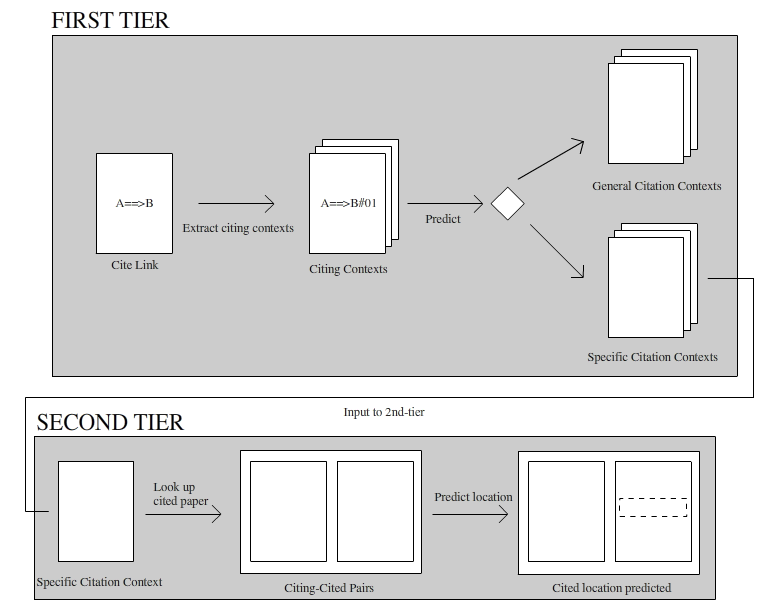
\includegraphics[scale=0.60]{./twotier}
  \caption{A Two-Tier Approach}
  \label{fig:twotier}
\end{figure}

\subsection{First Tier}
\paragraph{}
The First Tier is our attempt to filter out the General citations. In this tier, we are performing a 2-class \textit{citation classification} task, which already is a challenging task in the research area of citation analysis. We are not interested in determining whether the citation is one of the 12 class as defined by \cite{teufel2009annotation}, but only whether it is General or Specific. For each cite link we extract its citing contexts. Then for these contexts we extract feature vectors in order to pass it into our prediction model. We adopt similar features that were presented in previous works on citation classification.

\subsubsection{First Tier Features}
\begin{enumerate}
\item Physical Features \\
We adopted the physical features as presented in \cite{dongensemble}. They are:
\begin{enumerate}
\item \textit{Location}: in which section the citing sentence is from.
\item \textit{Popularity}: no. of citation marks in the citing sentence.
\item \textit{Density}: no. of unique citation marks in the citing sentence and its neighbour sentences.
\item \textit{AvgDens}: the average of Density among the citing and neighbour sentences.
\end{enumerate}

\item Number Density \\
A numerical feature that measures the density of numerical figures in the citing context. The intuition is that Specific citations tend refer to evaluation results in the cited paper. E.g. ``...Nivre and Scholz (2004) obtained a precision of 79.1\%...".

\item Publishing Year Difference \\
A numerical feature that represents difference in the publishing year between the citing and cited paper. The intuition is that higher difference suggests cited paper is older and presented a fundamental idea, and thus cited for General purposes.

\item Citing Context's Average \url{tf-idf} Weight \\
A numerical feature that indicates the amount of \textit{valuable} (as determined by \url{tf-idf} \cite{irtextbook}) words in the citing context. Higher values suggest important words and thus specific keywords.

%Tao: You'd better put the complete cue words list in the appendix
\item Cue Words \\
Another numerical feature adopted from \cite{dongensemble}, that computes the amount of cue words (pre-defined manually by us) that appear in the citing sentence and its neighbour sentences. We defined 2 classes of cue words: Cue-General and Cue-Specific. Cue-General $ = \{proposed, introduced, sketched, discussed, suggested\ldots \}$ and Cue-Specific $ = \{obtained, scored, precision, probabilities, experimental\ldots \}$. These cue words are selected based on the examples we observed in our training corpus.
\end{enumerate}
From our training corpus we extracted these features to build our First Tier Model for prediction.

\subsection{Second Tier}
\paragraph{}
In our Second Tier, it is another abstraction of our problem. It is independent from the First tier. We assume all the inputs into the second tier are Specific citations, and then we attempt to predict which of the fragments in the cited paper is the cited fragment.

\subsubsection{Second Tier Features}
\begin{enumerate}
\item Surface Matching \\
A numerical feature that measures the amount of word overlap between the citing sentence and a fragment in the cited paper.

\item Number Near-Miss \\
A numerical feature that measures the amount of numerical figures overlap between the citing sentence and a fragment in the cited paper. This feature will preprocess each fragment, rounding numerical figures or converting to percentage values, when it tries to match the numerical figures in the citing sentence. The intuition for this feature is from our observations that most Specific citations refer to evaluation results in the cited paper.

\item Bigrams Matching \\
A numerical feature that measures the amount of bigrams overlap between the citing sentence and a fragment in the cited paper. This feature is to preserve word order when comparing the citing sentence and the fragment. This feature is also targeted at Specific citations that refer to the cited paper for term definitions and quoting.

\item Cosine Similarity \\
A common numerical feature used in information retrieval tasks to measure similarity between the query and a candidate document. In our case, citing sentence and the fragment.
\end{enumerate}
Similarly we extracted these features from our training data to build our Second Tier Model for prediction.
%\chapter{Evaluation}
\label{evaluation}
\paragraph{}
We performed 2 evaluations, one for each tier as described early in Chapter \ref{twotierapproach}. We are able to do this because the tiers are independent of each other.

\section{Results - First Tier}
\paragraph{}
Recall that we have 275 annotated cite links, either General ($g$) or Specific ($s$), and that we have very limited instances of Specific cite links, a situation mentioned in \cite{li2010negative}, that we have a highly unbalanced ratio between General instances and Specific instances. So for our evaluation, we first gathered all Specific instances, and then randomly select General instances, twice the number of Specific instances. Out of these 84 instances, we have $1:2$ ratio of Specific vs General instances.

\paragraph{}
We trained our model using various classifiers, and then performed \url{Leave-One-Out} evaluation using the 84 instances. In other words, in one round of evaluation we predict 84 times. For each classifier, we performed 10 rounds of evaluation and we compute the average score for each round. Table \ref{tab:firsttieresults} summarises the accuracy for each classifier.

\begin{table}[h]
	\center
	\begin{tabular}{| l | l | l |}
		\hline
		\textsc{SVM} & \textsc{NaiveBayes} & \textsc{DecisionTree} \\
		\hline
		
	\end{tabular}
	\caption{Annotation Statistics}
	\label{tab:firsttieresults}
\end{table} %combined together with chapter 3
\chapter{Conclusion}
\label{conclusion}
\paragraph{}
We touched on a new task for citation analysis, Citation Provenance. In this task, we are trying to first determine whether a in-line citation is General or Specific, and second, if Specific, to locate where in the cited paper is the referenced information for the citation itself.

\paragraph{}
One of the challenges in this task is the highly unbalanced ratio between General versus Specific citations, i.e. Specific citations are very rare. Also, the annotation task is very challenging and would require experienced researchers who understands the content of the papers to be annotated.

\paragraph{}
We presented a two-tier approach towards this problem. With the first acting as a filter to separate the General citations from the Specific ones and the second one to predict which of the fragments in the cited paper are referenced by the citation. We arranged for our training set to have a balanced ratio of General versus Specific instances, so that the results would reflect the extent our approach is able to differentiate the 2 types of citations we defined. We evaluated our approach on 3 classifiers and we were able to obtain promising results. 
%\chapter{Discussion}
\label{discussion}
\paragraph{}
Citation Provenance is a task that has relatively little developments done on it. In our paper we attempt to define the nature of the problem, and presented a possible approach to tackle it. One of the main challenges we had with this task is the limited number of Specific citations in scientific papers. Teufel et al. showed that the percentage of neutral citations was 62.7\%. We can say that the percentage of General citations is at least as much, because our definition of a Specific citation is much more restricted compared to the 12 classes defined in \cite{teufel2009annotation}. We observed, and conclude that in general research \& scientific papers, most citations are neutral and General.

\paragraph{}
We argue, that even though the percentage of Specific citations is very low and that the value of applications that perform such task seems low, citation provenance would prove to be an important reading tool that helps readers understand and navigate between papers that are linked via citations. We support with evidence the validity of our claim, that our prototype application submitted as part of the \url{Code For Science} 2012 competition organised by Elsevier was well received among the judging panel that consisted of professionals from fields related to information technology and libraries.

%Tao: Include the actual link (http://www.codeforscience.com/singapore) of codeforscience competition  %combined together with chapter 5


\bibliographystyle{socreport}
\bibliography{bibsource}

\appendix

\end{document}
